% !TEX root = ./main.tex
\documentclass[main.tex]{subfiles}
\begin{document}


\subsection{What Is a Prime?}
Prime numbers are defined as \textit{positive integers} which only have the factors 1 and itself. Thus $4$ is not a prime since $4 = 2 * 2$. On the other hand $5$ is a prime since the only divisors of $5$ is $1$ and $5$. An exception to this definition is $1$, since it's the first natural number.

If a number, $n$, is not prime, it is referred to as a \textit{composite number}.

\subsection{Mersenne Primes}
A mersenne prime is a prime that can be written as $2^{p}-1$ where $p$ is also a prime number. An example of this is $2^5-1$ which equals to $127$ which is a prime. Apart from having a connection to perfect numbers, mersenne primes are useful when it comes to finding larger and larger primes, because of their special properties which the computer programs exploit. This is undoubtedly the reason the eight largest primes are all mersenne primes. 

\subsection{The Fundamental Theory of Arithmetic}
The Fundamental Theory of Arithmetic \cite{theorem:arithmetic} states that all integers greater than $1$ is either a prime, or can be expressed as a product of primes in a unique way. This means that all natural numbers, except for $1$, has its own factorization containing only primes, unless it is a prime itself.
\newline
\\*
Important to know is that there is an infinite amount of primes. The proof is a quite easy by contradiction, but nonetheless beautiful:

\begin{mdframed}
    Assume that there is a finite amount of primes and make a list of them:

    $p_1, p_2, p_3, p_4, p_5, ...$ 
    \newline
    \\*
    Let the constant $Q$ be the product of all the primes in the list and add 1:

    $Q = p_1 * p_2 * p_3 * ... + 1$
    \newline
    \\*
    According to the fundamental theorem of arithmetic, $Q$ must be a prime since none of the primes in the list divide $Q$ evenly because of the $1$; therefore making the list incomplete and proving that you cannot make a finite list of all primes. 
\end{mdframed}

\subsection{The Prime Number Theorem}
The Prime Number Theorem \cite{theorem:prime_num} describes approximately how many primes there are less than or equal to a given number. The function $\pi(N) \sim \frac{N}{ln(N)}$ gives the expected amount of primes below a certain $N$. Graphing this function shows that primes become less common for greater $N$.

\begin{figure}[ht]
    \begin{center}
        \begin{tikzpicture}
            \begin{axis}[
                axis lines = left,
                xlabel = $N$,
                ylabel = {},
            ]
            \addplot [
                domain=0:100000, 
                samples=100, 
                color=red,
            ]{x/ln(x)};
            \addlegendentry{$\frac{N}{ln(N)}$}
            
            \addplot [
                domain=0:100000, 
                samples=100, 
                color=blue,
            ]{x};
            \addlegendentry{$N$}
            \end{axis}
        \end{tikzpicture}
    \end{center}
\caption{The graph of $\pi(N)$ and $N$ from $0$ to $10^{5}$ letting us compare the relationship between the number $N$ and the approximate amount of primes below it.}
\end{figure}

This proves that primes do not show up linearly, meaning a computer that is twice as powerful will \textit{not} produce twice as many primes. Instead, the most important and crucial part of generating and verifying primes is the optimization of the \textit{algorithms}.

\subsection{Time Complexity}

Time complexity \cite{theorem:time_comp} is a concept within computer science, which describes the approximate time for a program to complete. The study will make heavy use of the Big O Notation \cite{theorem:big_O}, which notates how the run time increases as the input size increases. For example, $O(N)$ will grow linearly with the input size. Increasing the input size by a factor of 10, will also increase the run time by a factor of 10, as such $O(10N)$. On the other hand, $O(log(n))$ grows logarithmically, which is far more efficient for bigger input sizes, as $O(log(N))$ is strictly smaller than $N$ for large enough values. The base for logarithms in the Big O Notation is not relevant. The proof as to why the base is irrelevant will not be provided by this study.
\newline
The amount of operations a modern computer can do is in the order of magnitude of $10^{9}$ per second. An operation is for example adding two numbers or storing a number in an array. 
\newline
Since the Big O Notation denotes the growth of the runtime as $\lim_{N\to\infty}$, two notations can be added together rather easily. For example, a program that has two bits of codes, one with $O(N)$ and another with $O(N^{2})$, will have an overall time complexity of $O(N^{2})$ since $N^{2}$ dominates for large values of $N$
\newline
\\*
The Big O Notation will be used to determine whether an algorithm with a large number, $n$, will succeed or run for a \textit{very long time}\footnote{Some programs will not finish until the sun explodes, which is quite impractical.}. Considering that the largest known prime is $24,862,048$ digits \cite{prime:largest_digits}, algorithms have to be efficient to perform a primality test. 

\subsubsection{Examples of Big O Notation}


\begin{figure}[ht]
    \begin{center}
        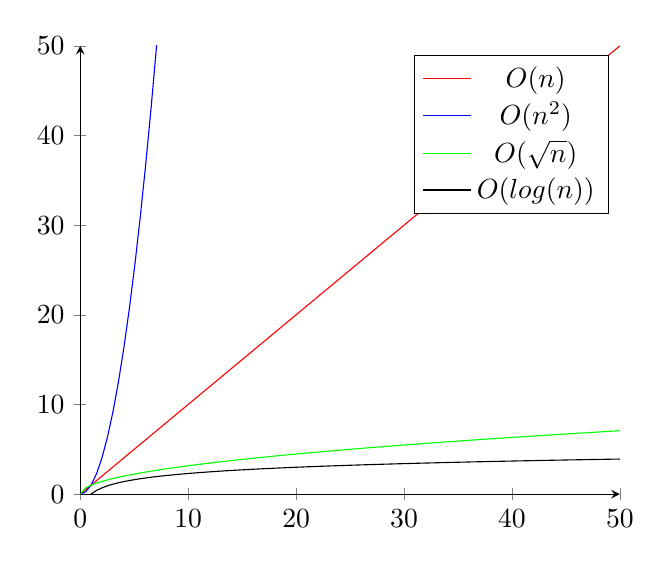
\begin{tikzpicture}
            \begin{axis}[
                axis lines = left,
                ymin=0, ymax=50,
                xlabel = {},
                ylabel = {},
            ]
            \addplot [
                domain=0:50, 
                samples=100, 
                color=red,
            ]{x};
            \addlegendentry{$O(n)$}
            
            \addplot [
                domain=0:50,
                samples=100, 
                color=blue,
                ]{x^2};
            \addlegendentry{$O(n^2)$}

            \addplot [
                domain=0:50,
                samples=100, 
                color=green,
                ]{sqrt(x)};
            \addlegendentry{$O(\sqrt{n})$}

            \addplot [
                domain=0:50,
                samples=100, 
                color=black,
                ]{ln(x)};
            \addlegendentry{$O(log(n))$}
            \end{axis}
        \end{tikzpicture}
    \end{center}
\caption{The graph does a lot of stuff. The graph does a lot of stuff. The graph does a lot of stuff. The graph does a lot of stuff. The graph does a lot of stuff. The graph does a lot of stuff. The graph does a lot of stuff.}
\end{figure}

\vspace{10mm}

A program that runs in $O(N)$ would be a function that inputs an integer $N$ and outputs every number up to $N$. This runs in $O(N)$ time because it does $1+N$ operations which results in $O(n)$:
\begin{python}
def linearTime(N):
    for number in range(N):
        print(number)
\end{python}

Since the program runs in $O(N)$ time, increasing the input by a factor of $10$ would also increase the number of operations done by a factor of $10$.
\newline
\\*
The second example is a program that runs in quadratic time, i.e. $O(N^{2})$. Compared to the first example, this program will print every number up to $N$, $N$ times.

\begin{python}
    def quadraticTime(N):
        for number in range(N):
            for number in range(N):
                print(number)
\end{python}

\vspace{10mm}

The third program describes $O(\sqrt{n})$. It is a simple program that sums all numbers up to $\sqrt{N}$.

\begin{python}
    from math

    def sqrtTime(N):
        sum = 0
        for number in range(math.isqrt(N)):
            sum += number
        print(sum)
\end{python}

\vspace{10mm}

The fourth and last example will be about $O(log (n))$. The algorithm that is used in this example is called \textit{Binary Search} \cite{algh:binary_search}. It's an algorithm used for quickly guessing a number between, for example, $1$ and $100$. Usually two players are required to play this guessing game, but with a computer the user will give an input that the computer will try to guess. The output will be the amount of "guesses" the algorithm performed.

\begin{python}
    def binarySearch():
        begin = int(input("The number will be between _ and _\n"))
        end = int(input())
        value = int(input("What value will you input?\n"))
        guesses = 0

        while True:
            guesses += 1
            mid = int((begin + end) / 2)
            if mid > value:
                end = mid - 1
            elif mid < value:
                begin = mid + 1
            else:
                break

    print(guesses)

\end{python}

\subsection{Deterministic vs. Probabilistic}
A deterministic test is a test that is a one-hundred percent definite test for primes, that gives no false positives or false negatives. It either returns true if the number being tested if prime, else it returns false. 

Probabilistic tests differ from deterministic tests by having a stochastic, random, factor in them. They are not one-hundred percent definite and therefore sometimes will give false positives or negatives. An example of a probabilistic test for the number $p$ would be to test a random number below $p$ and see if it divides $p$ evenly. This test would give a lot of false positives, because even if $p$ is composite, not all numbers below it will divide it. The accuracy of the test, i.e. the probability that it returns a correct answer, could be increased by increasing the amount of unique factors tested. This will be an important fact in the Fermat and Miller-Rabin primality tests. There, the variable $k$ will be used to specify the number of rounds the test will run. 

\subsection{Algorithms}

\subsubsection{Brute-force}
The brute force method is arguably the simplest of all algorithms. This algorithm tests all the numbers, $n$, between $2$ and $p-1$ and checks if $n$ satisfies $n \equiv 0 \Mod{p}$, which makes $n$ a divisor of $p$ and therefore $p$ is definitely not prime. If the loop, however, completes without finding any divisors of $p$, then $p$ is definitely prime. The pros of this method are that it is simple to understand, and that it is a definite test; $p$ is prime if and only if there are no divisors except for 1 and $p$ itself. The big con is that this algorithm is slow. It runs in $O(N)$ time which is the slowest of all algorithms which will be tested in this essay. 

\begin{python}
    Insert code here
\end{python}

\subsubsection{Smart Brute-force}
The smart brute force is also a brute force algorithm, but it utilizes some of the properties of primes. Since a prime can never have the factor $2$ in them, it is sufficient to only test $2$ and the odd numbers. On top of this, the smart brute force only tests numbers up to and including $\sqrt{p}$. This is because, assuming that $p$ is composite, it must have at least 2 factors. If there exists a factor larger than $\sqrt{p}$, it must have already been tested. This algorithm will run in $O(\sqrt(n))$ time, which is much faster than the original brute force.

\begin{python}
    Insert code here
\end{python}

\subsubsection{Lucas-Lehmer}
The Lucas-Lehmer algorithm is a deterministic primality test that only works for Mersenne numbers. It takes advantage of a special property of Mersenne numbers:

\begin{mdframed}
    For some $p>2$, $M_p=2^p-1$ is prime if and only if $M_p$ divides $S_{p-2}$ where $S_0=4$ and $S_k=(S_{k-1})^2-2$ for $k>0$. 
\end{mdframed}

There exists a proof for this, which will not be covered by this essay.

The Lucas-Lehmer test has helped the GIMPS (Great Internet Mersenne Prime Search) to find many of the largest primes known to man. This because the time complexity of this test is much faster compared to the other tests. Another advantage it has over some of the other tests, is that it is deterministic.

\subsubsection{Fermat}
* The history about the algorithm. Prob or Det? Who made it? Awards?
* Why is it relevant? Time complexity?
* How does it work?


\subsubsection{Miller–Rabin}
The Miller-Rabbin primality test \cite{algh:miller}, first discovered by Russian
mathematician M. M. Artjuhov in 1967, is an algorithm that has two versions. One
that is deterministic, and the other probabilistic. The deterministic version is
conditional, meaning that it relies on an unproven theorem, in this case, the
extended Riemann hypothesis \cite{riemann}. However, the probabilistic version is
unconditional, meaning that it does not depend on an unproven theorem. This
makes the probabilistic version reliable. If the extended Riemann
hypothesis were to be disproved, the deterministic version would fall apart.
Therefore, the probabilistic is chosen for this study. % probabilistska är väl snabbare också?
\newline
\\*
The Miller-Rabin primality test is considered to be one of the fastest
algorithms to verify if an $n$ is prime or not. The time complexity for the
probabilistic version is $O(k log^{3}(n))$, where $k$ is the amount of rounds
the algorithm will perform. 
\newline
\\*
insert how it works here
\end{document}
